\section{二分圖判定}
    \subsection{概念}
    有沒有一種方式可以將圖中的點分成兩組,使組內沒有成員之間的邊。如下圖。

    \begin{figure}[ht]
        \centering
        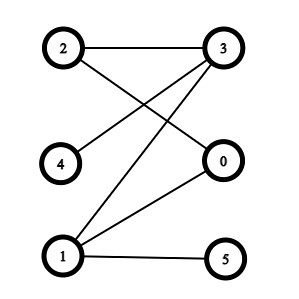
\includegraphics[width=0.5\textwidth]{../Images/Graph3.jpg}
        \caption{二分圖}
    \end{figure}

    \textbf{判別方法}

    想像將圖上色,用 12 表示,相鄰的點都用不同色,如果沒有辦法使用就代表這
    張圖不是二分圖。實作上,如果對方已經跟你有相同顏色表示沒有辦法。

    \subsection{實作}

\begin{lstlisting}[caption=二分圖判定]
int color[N];
bool isBipartiteGraph(int n){
    for(auto u:g[n]){
        // 用 color==0 代替 bool isv[N];
        if(color[u]==0){
            // 有一個邪門的技巧 color[u]=color[n]^3;
            color[u]=color[n]%2+1;
            if(!isBipartiteGraph(u))
                return false;
        }else if(color[u]==color[n]){
            return false;
        }
    }
    return true;
}
\end{lstlisting}

    \subsection{範例與練習}

    \problem TIOJ 1209 圖論之二分圖測試

    \textbf{題目敘述}

    給你一個圖(Graph),請問這個圖是否為一個二分圖(bipartite graph)?

    所謂的二分圖,就是存在一種分法,把所有頂點分成兩個點集X和Y,其中X以及Y內部的頂點互不相鄰。

    \textbf{輸入說明}

    輸入可能包含多筆測試資料。

    每筆測試資料的第一列有兩個整數$n,m(1 \le n \le 40,000,0 \le m \le 500,000)$,
    分別代表一個圖的點數和邊數。點的編號是從1到n。

    接下來有m列,每列有兩個以空白隔開的正整數,代表一條邊所連的兩個端點編號。
    當$n=m=0$時代表輸入結束。

    \textbf{輸出說明}

    對於每筆測試資料,若該圖是二分圖,請輸出Yes,否則輸出No。

    \textbf{範例測試}

    \begin{tabular}{|m{7cm}|m{7cm}|}
        \hline
        範例輸入 1 & 範例輸出 1 \\
        \hline
        \verb|3 2|  & \verb|Yes| \\
        \verb|2 3|  & \verb|No| \\
        \verb|1 2|  &\\
        \verb|3 3|  &\\
        \verb|1 2|  &\\
        \verb|2 3|  &\\
        \verb|3 1|  &\\
        \verb|0 0|  &\\
        \hline
    \end{tabular}

    \problem ZJ g598 真假子圖

    \textbf{題目敘述}

    情報調查局內有 
    n 個工作人員,調查局負責人將這些人秘密分成兩組 
    A 和 B 並不讓其他人知道,並將合作名單分配給組長,合作名單是由很多個 pair 組成,每個 pair 
    $x,y$ 代表 x 和 y 需要合作完成任務,
    並且保證 x 和 y 不會同時在 A 組或是同時在 B 組。

    組長不小心將這個合作名單分配遺失,僅剩下其中 
    m 個 pair,為了要復原這些失去的資料,組長派出了另外 
    p個調查員編號1到 
    p去調查這個合作關係,每一個調查員都會回傳恰好k個 pair 的資料回來

    有些調查員回傳的資料和組長手上的資料會產生矛盾
    (意即加上這 k個 pair 和組長手上存留的m個 pair 會使得這些人是被分成 
    A,B兩組這件事產生矛盾),請將回傳錯誤結果的調查員編號由小到大輸出出來,
    保證至少一個且最多三個。

    另外保證若調查員的 k 個 pair 的結果和組長存留的 m 個 pair 不會產生矛盾,則保證調查員的資料一定和原本 
    A,B分組吻合。

    \textbf{輸入說明}

    第一行先輸出兩個正整數 
    n和m 

    第二行來有 
    2m個非負整數兩兩形成一個數對,表示目前還留存的 
    m個 pair

    第三行有兩個正整數 
    p和k 

    並且接下來的 
    p行每行有 
    2k個非負整數, 兩兩形成一對代表某個調查員找到的 
    k個 pair

    \textbf{輸出說明}

    由小到大輸出會形成矛盾的調查員編號,每個編號各自獨立一行。

    \textbf{範例測試}

    \begin{tabular}{|m{7cm}|m{7cm}|}
        \hline
        範例輸入 1 & 範例輸出 1 \\
        \hline
        \verb|7 5|  & \verb|2| \\
        \verb|0 1 0 2 1 3 2 3 4 5|  & \\
        \verb|2 3|  &\\
        \verb|0 6 2 4 3 6|  &\\
        \verb|0 6 0 3 3 5|  &\\
        \hline
    \end{tabular}

    \problem AtCoder ABC 282D Make Bipartite 2

    \textbf{題目敘述}

    給定一個包含$N$個頂點和$M$條邊(一個簡單圖不包含自環或多邊)的簡單無向圖$G$。對於$i=1,2,…,M$,第$i$條邊連接頂點$u_i$和頂點$v_i$。

    請打印滿足以下兩個條件的整數對$(u,v)$的數量,其中$1\leq u<v\leq N$。

    圖$G$沒有連接頂點$u$和頂點$v$的邊。

    在圖$G$中添加一條連接頂點$u$和頂點$v$的邊會得到一個二部圖。

    $2\leq N\leq 2\times 10^5$

    $0\leq M\leq \min{2\times 10^5, N(N-1)/2}$

    $1\leq u_i, v_i\leq N$

    \textbf{輸入說明}

    輸入以以下格式從標準輸入中給出。

    $N$ $M$

    $u_1$ $v_1$

    $u_2$ $v_2$

    $\vdots$

    $u_M$ $v_M$

    \textbf{輸出說明}

    輸出答案。

    \textbf{範例測試}

    \begin{tabular}{|m{7cm}|m{7cm}|}
        \hline
        範例輸入 1 & 範例輸出 1 \\
        \hline
        \verb|5 4|  & \verb|2| \\
        \verb|4 2|  & \\
        \verb|3 1|  &\\
        \verb|5 2|  &\\
        \verb|3 2|  &\\
        \hline
    \end{tabular}